\documentclass[12pt, twoside]{article}
\usepackage[letterpaper, margin=1in, headsep=0.5in]{geometry}
\usepackage[english]{babel}
\usepackage[utf8]{inputenc}
\usepackage{amsmath}
\usepackage{amsfonts}
\usepackage{amssymb}
\usepackage{tikz}
\usetikzlibrary{quotes, angles}
\usepackage{graphicx}
%\usepackage{pgfplots}
%\pgfplotsset{width=10cm,compat=1.9}
%\usepgfplotslibrary{statistics}
%\usepackage{pgfplotstable}
%\usepackage{tkz-fct}
%\usepackage{venndiagram}

\usepackage{fancyhdr}
\pagestyle{fancy}
\fancyhf{}
\renewcommand{\headrulewidth}{0pt} % disable the underline of the header

\fancyhead[RE]{\thepage}
\fancyhead[RO]{\thepage \\ Name: \hspace{3cm}}
\fancyhead[L]{BECA / Dr. Huson / Geometry 10th Grade\\* Unit 2: Midpoints and distance \\ 
16 September 2019}

\begin{document}
  \subsubsection*{2.1 Do Now: Exam review}
 % \emph{Study your errors. For each, write a note to yourself: what you need to do differently.}
  %  \vspace{0.5cm}
    \begin{enumerate}
      \item Complete the construction of an equilateral triangle and complete the six steps.
      \begin{enumerate}
        \item Given the line segment $\overline{MN}$.
        \bigskip
        \item Construct circle $M$ with radius $MN$.
        \bigskip
        \item Construct circle $\rule{2cm}{0.15mm}$  with radius $MN$. \bigskip
        \item Label the intersection $P$ of the two circles.
        \bigskip
        \item Draw line segment $\overline{MP}$ and line segment $\rule{2cm}{0.15mm}$
        \bigskip
        \item $\triangle MNP$ is equilateral.
      \end{enumerate}
      \vspace{7cm}
      \begin{center}
      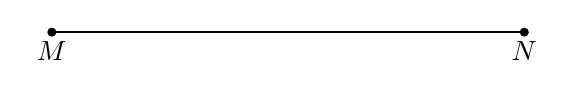
\begin{tikzpicture}
        \draw [-, thick] (0,0)--(6,0);
        \draw [fill] (0,0) circle [radius=0.05] node[below]{$M$};
        \draw [fill] (6,0) circle [radius=0.05] node[below]{$N$};
      \end{tikzpicture}
      \end{center}
    \end{enumerate}
\end{document}
